{
\LinesNumberedHidden
  \def\bb#1{$\textit{bb}_{#1}$}

\chapter{Loop tree and induction variables \Author{S. Pop \andAuthor A. Cohen}}
\label{chapter:loop_tree}
\inputpath[fig]{part3}{loop_tree}
\inputprogress


\providecommand{\SSA}{SSA}
\providecommand{\CFG}{CFG}
\providecommand{\loopphi}{loop-$\phi$}
\providecommand{\closephi}{close-$\phi$}
\providecommand{\CHREC}[1]{\{#1\}}

This\index{induction variable recognition} chapter presents an extension of the \SSA{} under which the extraction of the reducible loop tree can be done only on the \SSA{} graph itself. 
This extension also captures reducible loops\index{reducible loop} in the CFG. 
This chapter first illustrates this property then shows its usefulness through the problem of induction variable recognition.

\section{Part of the \CFG{} and Loop Tree can be exposed from the \SSA{}}

During the construction of the \SSA{} representation based on a \CFG{} representation, a large part of the \CFG{} information is translated into the \SSA{} representation. 
As the construction of the \SSA{} has precise rules to place the \phinodes in special points of the \CFG{} (i.e., at the merge of control-flow branches), by identifying patterns of uses and definitions, it is possible to expose a part of the \CFG{} structure from the \SSA{} representation.

Furthermore, it is possible to identify higher level constructs inherent to the \CFG{} representation, such as strongly connected components of basic blocks (or reducible loops), based only on the patterns of the \SSA{} definitions and uses. 
The induction variable analysis presented in this chapter is based on the detection of self references in the \SSA{} representation and on its characterization.

This first section shows that the classical \SSA{} representation is not enough to represent the semantics of the original program. 
We will see the minimal amount of information that has to be added to the classical \SSA{} representation in order to represent the loop information: 
similar to the $\phiexit$-function used in the Gated \SSA{} presented in Chapter~\ref{chapter:vsdg}, the loop closed \SSA{} form adds an extra variable at the end of a loop for each variable defined in a loop and used after the loop.

\subsection{An \SSA{} representation without the \CFG{}}
In the classic definition of the \SSA{}, the \CFG{} provides the skeleton of the program: 
basic blocks contain assignment statements defining \SSA{} variable names, and the basic blocks with multiple predecessors contain \phinodes. 
Let us look at what happens when, starting from a classic \SSA{} representation, we remove the \CFG{}.

In order to remove the \CFG{}, imagine a pretty printer function that dumps only the arithmetic instructions of each basic-blocks and skips the control instructions of an imperative program by traversing the \CFG{} structure in any order. 
Does the representation, obtained from this pretty printer, contains enough information to enable us to compute the same thing as the original program?~\footnote{To simplify the discussion, we consider the original program to be free of side effect instructions.}
%
Let us see what happens with an example in its \CFG{} based \SSA{} representation:

% \begin{center}
  % \begin{minipage}{.8\linewidth}
% \begin{verbatim}
% bb_1 (preds = {bb_0}, succs = {bb_2})
% {
  % a = #some computation independent of b
% }
% bb_2 (preds = {bb_1}, succs = {bb_3})
% {
  % b = #some computation independent of a
% }
% bb_3 (preds = {bb_2}, succs = {bb_4})
% {
  % c = a + b;
% }
% bb_4 (preds = {bb_3}, succs = {bb_5})
% {
  % return c;
% }
% \end{verbatim}
\centerline{\tikzfigure{example1}}
% \end{minipage}
% \end{center}

\noindent
After removing the \CFG{} structure, listing the definitions in an arbitrary order, we could obtain this:

\begin{algorithm}[H]
% \begin{verbatim}
% return c;
% b = #some computation independent of a
% c = a + b;
% a = #some computation independent of b
% \end{verbatim}
\Return $c$\;
$b \gets \ldots$ \Comment*{some computation independent of a}
$c \gets a + b$\;
$a \gets \ldots$ \Comment*{some computation independent of b}
\end{algorithm}


\noindent
And this \SSA{} code is enough, in the absence of side effects, to recover an order of computation that leads to the same result as in the original program. 
For example, the evaluation of this sequence of statements would produce the same result:

% \begin{center}
  % \begin{minipage}{.8\linewidth}
% \begin{verbatim}
% b = #some computation independent of a
% a = #some computation independent of b
% c = a + b;
% return c;
% \end{verbatim}
% \end{minipage}
% \end{center}

\begin{algorithm}[H]
% \begin{verbatim}
% return c;
% b = #some computation independent of a
% c = a + b;
% a = #some computation independent of b
% \end{verbatim}
$b \gets \ldots$ \Comment*{some computation independent of a}
$a \gets \ldots$ \Comment*{some computation independent of b}
$c \gets a + b$\;
\Return $c$\;
\end{algorithm}



\subsection{Natural loop structures on the \SSA{}}
We will now see how to represent the natural loops in the \SSA{} form by systematically adding extra $\phi$-nodes at the end of loops, together with extra information about the loop exit predicate.
Supposing that the original program contains a loop:

\centerline{\tikzfigure{example2}}
%% \begin{center}
%%   \begin{minipage}{.8\linewidth}
%% \begin{verbatim}
%% bb_1 (preds = {bb_0}, succs = {bb_2})
%% {
%%   x = 3;
%% }
%% bb_2 (preds = {bb_1, bb_3}, succs = {bb_3, bb_4})
%% {
%%   i = phi (x, j)
%%   if (i < N) goto bb_3 else goto bb_4;
%% }
%% bb_3 (preds = {bb_2}, succs = {bb_2})
%% {
%%   j = i + 1;
%%   goto bb_2;
%% }
%% bb_4 (preds = {bb_2}, succs = {bb_5})
%% {
%%   k = phi (i)
%% }
%% bb_5 (preds = {bb_4}, succs = {bb_6})
%% {
%%   return k;
%% }
%% \end{verbatim}
%% \end{minipage}
%% \end{center}

\noindent
Pretty printing, with a random order traversal, we could obtain this \SSA{} code:
%% \begin{center}
%%   \begin{minipage}{.8\linewidth}
%% \begin{verbatim}
%% x = 3;
%% return k;
%% i = phi (x, j)
%% k = phi (i)
%% j = i + 1;
%% \end{verbatim}
%% \end{minipage}
%% \end{center}

\begin{algorithm}[H]
$x\gets 3$\;
\Return $k$\;
$i\gets \phi(x,j)$\;
$k\gets\phi(i)$\;
$j\gets i+1$\;
\end{algorithm}

We can remark that some information is lost in this pretty printing: 
the exit condition of the loop have been lost. 
We will have to record this information in the extension of the \SSA{} representation. 
However, the loop structure still appears through the cyclic definition of the induction variable $i$. 
To expose it, we can rewrite this \SSA{} code using simple substitutions, as:

\begin{algorithm}[H]
$i\gets \phi(3,i+1)$\;
$k\gets\phi(i)$\;
\Return $k$\;
\end{algorithm}

%% \begin{center}
%%   \begin{minipage}{.8\linewidth}
%% \begin{verbatim}
%% i = phi (3, i + 1)
%% k = phi (i)
%% return k;
%% \end{verbatim}
%% \end{minipage}
%% \end{center}

\noindent
Thus, we have the definition of the \SSA{} name $i$ defined in function of itself. 
This pattern is characteristic of the existence of a loop. 
We can remark that there are two kinds of \phinodes used in this example:
\begin{itemize}
\item {\bf \loopphi{} nodes}  ``$i = \phi (x, j)$''\index{$\phientry$-node} (also denoted $i = \phientry (x, j)$ as in Chapter~\ref{chapter:vsdg}) have an argument that contains a self reference $j$ and an invariant argument
$x$: 
here the defining expression ``$j = i + 1$'' contains a reference to the same \loopphi{} definition $i$, while $x$ (here $3$) is not part of the circuit of dependencies that involves $i$ and $j$.
Note that it is possible to define a canonical \SSA{} form by limiting the number of arguments of \loopphi{} nodes to two.
\item {\bf \closephi{} nodes} ``$k = \phiexit (i)$''\index{$\phiexit$-node} (also denoted $k = \phiexit (i)$ as in Chapter~\ref{chapter:vsdg}) capture the last value of a name defined in a loop. 
Names defined in a loop can only be used within that loop or in the arguments of a \closephi{} node (that is ``closing'' the set of uses of the names defined in that loop).
In a canonical \SSA{} form it is possible to limit the number of arguments of \closephi{} nodes to one.
\end{itemize}

\subsection{Improving the \SSA{} pretty printer for loops}
As we have seen in the above example, the exit condition of the loop disappeared during the basic pretty printing of the \SSA{}. 
To capture the semantics of the computation of the loop, we have to specify in the \closephi{} node, when we exit the loop so as to be able to derive which value will be available in the end of the loop. 
With our extension that adds the loop exit condition to the syntax of the \closephi{}, the \SSA{} pretty printing of the above example would be:

\begin{algorithm}[H]
$x\gets 3$\;
$i\gets \phientry(x,j)$\;
$j\gets i+1$\;
$k\gets\phiexit(i\geq N, i)$\;
\Return $k$\;
\end{algorithm}

%% \begin{center}
%%   \begin{minipage}{.8\linewidth}
%% \begin{verbatim}
%% x = 3;
%% i = loop-phi (x, j)
%% j = i + 1;
%% k = close-phi (i >= N, i)
%% return k;
%% \end{verbatim}
%% \end{minipage}
%% \end{center}
So $k$ is defined as the ``first value'' of $i$ satisfying the loop
exit condition, ``$i \geq N$''.  In the case of finite loops, this is well defined as being the first element satisfying the loop exit condition of the sequence defined by the corresponding \loopphi{} node.

In the following, we will look at an algorithm that translates the
\SSA{} representation into a representation of polynomial functions,
describing the sequence of values that \SSA{} names take during the execution of a loop. 
The algorithm is restricted to the loops that are reducible. 
All such loops are labeled. 
Note that irreducible control flow is not forbidden: 
only the loops carrying self-definitions must be reducible.

\section{Analysis of Induction Variables}

The purpose of the induction variables analysis is to provide a characterization of the sequences of values taken by a variable during the execution of a loop. 
This characterization can be an exact function of the canonical induction variable of the loop (i.e., a loop counter that starts at zero with a step of one for each iteration of the loop) or an approximation of the values taken during the execution of the loop represented by values in an abstract domain. 
In this section, we will see a possible characterization of induction variables in terms of sequences. 
The domain of sequences will be represented by {\em chains of recurrences}\index{chain of recurrences}: 
as an example, a canonical induction variable with an initial value $0$ and a stride $1$ that would occur in the loop with label $x$ will be represented by the chain of recurrence $\CHREC{0, +, 1}_x$.

\subsection{Stride detection}

The first phase of the induction variables analysis is the detection of the strongly connected components of the \SSA{}. 
This can be performed by traversing the use-def \SSA{} chains\index{use-def chain} and detecting that some definitions are visited twice. 
For a self referring use-def chain, it is possible to derive the step of the corresponding induction variable as the overall effect of one iteration of the loop on the value of the \loopphi{} node. 
When the step of an induction variable depends on another cyclic definition, one has to further analyze the inner cycle. 
The analysis of the induction variable ends when all the inner cyclic definitions used for the computation of the step are analyzed. 
Note that it is possible to construct \SSA{} graphs with strongly connected components that are impossible to characterize with the chains of recurrences. 
This is precisely the case of the following example that shows two inter-dependent circuits, the first that involves $a$ and $b$ with step $c+2$, and the second that involves $c$ and $d$ with step $a+2$. 
This leads to an endless loop, which must be detected.

\begin{algorithm}[H]
$a\gets \phientry(0,b)$\;
$c\gets \phientry(1,d)$\;
$b\gets c+2$\;
$d\gets a+3$\;
\end{algorithm}
%% \begin{center}
%%   \begin{minipage}{.8\linewidth}
%% \begin{verbatim}
%% a = loop-phi-x (0, b)
%% c = loop-phi-x (1, d)
%% b = c + 2
%% d = a + 3
%% \end{verbatim}
%% \end{minipage}
%% \end{center}

% \begin{figure}[h]
  % \begin{center}
    % 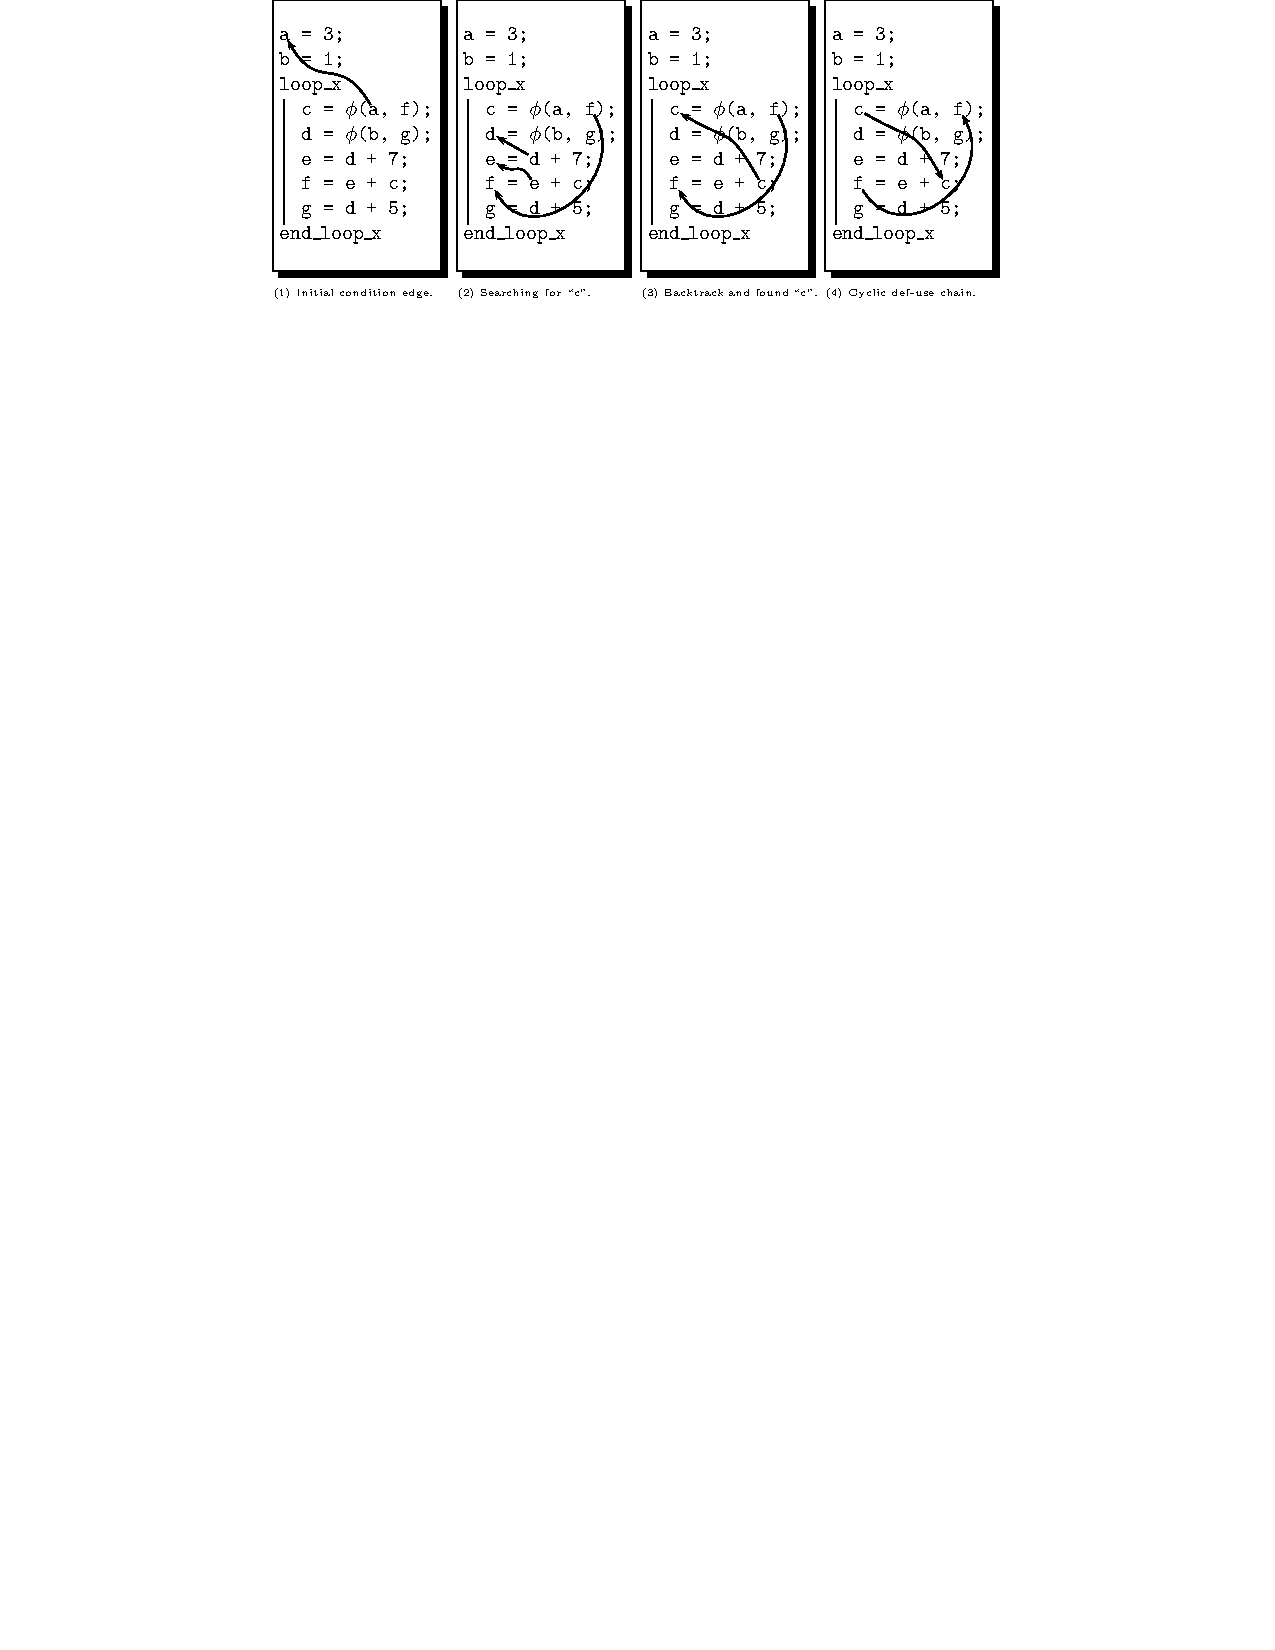
\includegraphics[width=1.2\textwidth]{iv_step}
  % \end{center}
  % \vspace{-50em}
  % \caption{Detection of the cyclic definition using a depth first
    % search traversal of the use-def chains.}
  \label{spop:fig:ivstep}
% \end{figure}

    \begin{figure}
\ifx\dousetikz\undefinedmacro
\warning{Low quality figure! Please compile with tikz.}
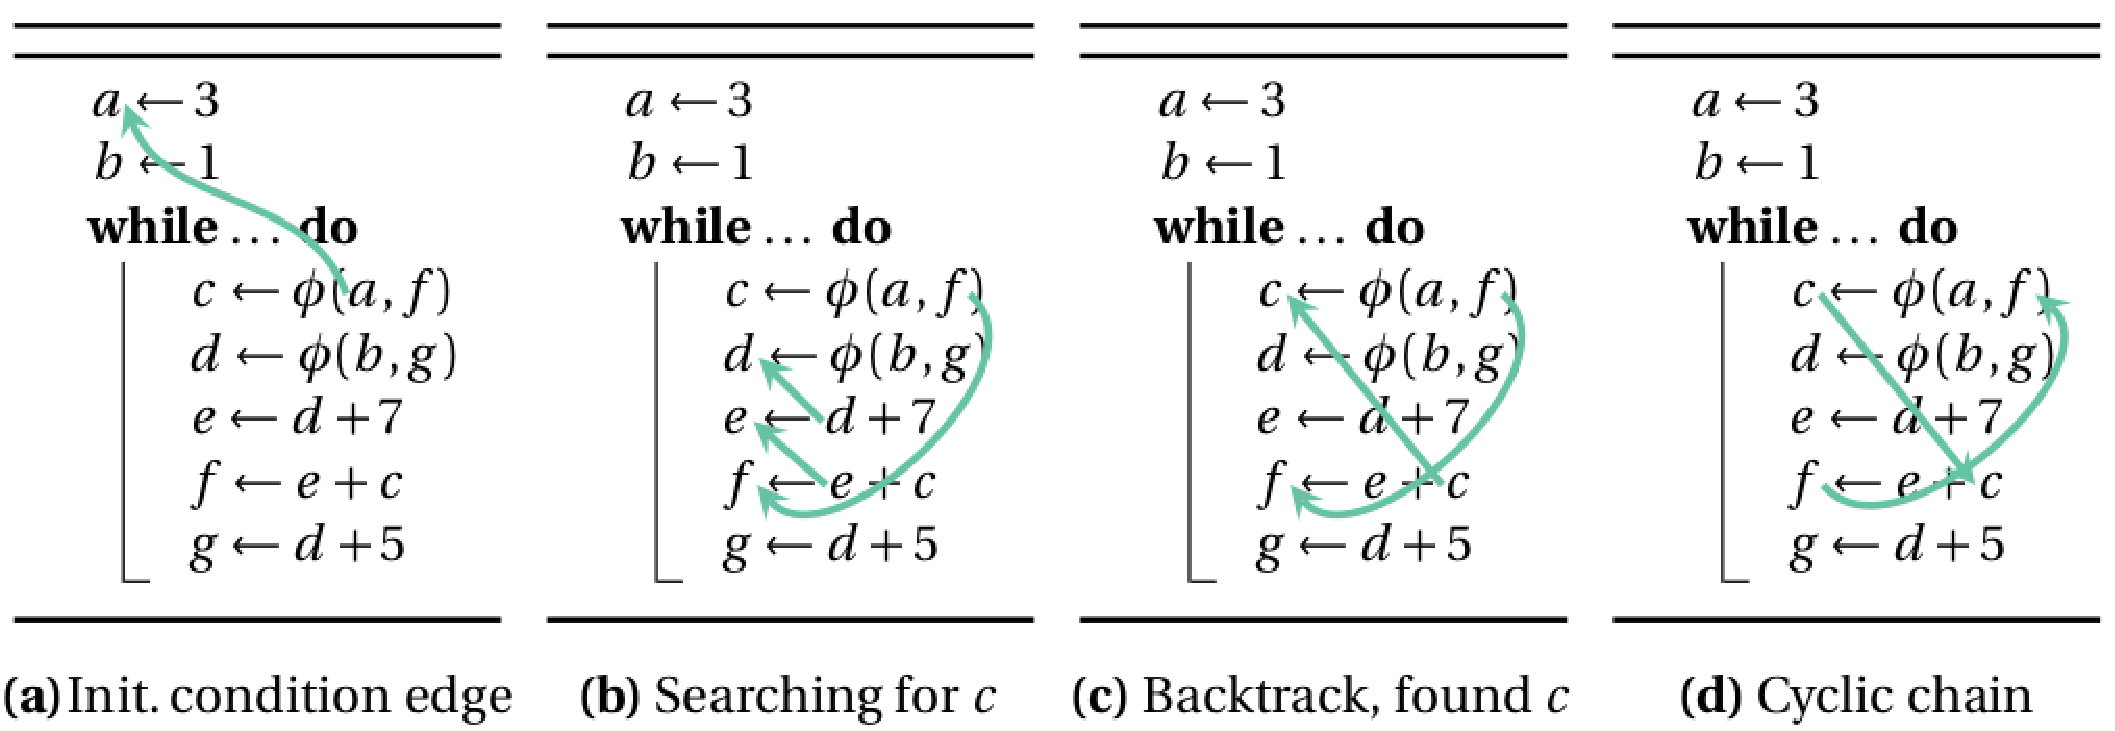
\includegraphics[width=\linewidth]{iv_step-tikz}
\else
{
  \def\tc#1{\tikz[remember picture,baseline=-.5ex]\coordinate(#1);}
  \foreach \ver/\cap in{1/\!Init.\,condition edge,2/Searching for 
    $c$,3/{Backtrack, found $c$},4/Cyclic chain}{
      \subfloat[\cap]{
        \begin{minipage}{.23\linewidth}
        \begin{algorithm}[H]
          $a \tc{da} \gets 3$\;
          $b \tc{db} \gets 1$\;
          \While{\ldots}{
            $c\tc{dc} \gets \phi(\tc{ua}a,f\tc{uf})$\;
            $d\tc{dd} \gets \phi(b,g)$\;
            $e\tc{de} \gets \tc{ud}d+7$\;
            $f\tc{df} \gets \tc{ue}e+\tc{uc}c$\;
            $g \gets d+5$\;
          }
        \end{algorithm}
        \end{minipage}
      }
%
      \begin{tikzpicture}[remember picture,overlay,
        dep/.style={\mycol{1},very thick,-stealth}
        ]
        \ifcase\ver\or
        \draw[dep] (ua) to[out=110,in=-70] (da);
        \or
        \draw[dep] (uf) to[out=-40,in=-50] (df);
        \draw[dep] (ud) -- (dd);
        \draw[dep] (ue) -- (de);
        \or
        \draw[dep] (uc) -- (dc);
        \draw[dep] (uf) to[out=-40,in=-50] (df);
        \or
        \draw[dep] (dc) -- (uc);
        \draw[dep] (df) to[out=-50,in=-40] (uf);
        \fi
      \end{tikzpicture}
    %
  }
}
\fi
  \caption{Detection of the cyclic definition using a depth first
    search traversal of the use-def chains.}
  \label{spop:fig:ivstep}
\end{figure}%
\ifx\dousetikz\undefinedmacro
\todo{Missing figure ! Please compile with tikz.}
\fi



Let us now look at an example, presented in Figure~\ref{spop:fig:ivstep}, to see how the stride detection works. 
The arguments of a \phinode are analyzed to determine whether they contain self references or if they are pointing towards the initial value of the induction variable. 
In this example, (a) represents the use-def edge that points towards the invariant definition. 
When the argument to be analyzed points towards a longer use-def chain, the full chain is traversed, as shown in (b), until a phi node is reached. 
In this example, the phi node that is reached in (b) is different to the phi node from which the analysis started, and so in (c) a search starts over the uses that have not yet been analyzed. 
When the original phi node is found, as in (c), the cyclic def-use chain provides the step of the induction variable: 
in this example, the step is ``$+ e$''. 
Knowing the symbolic expression for the step of the induction variable may not be enough, as we will see next, one has to instantiate all the symbols (``$e$'' in the current example) defined in the varying loop to precisely characterize the induction variable.

\subsection{Translation to chains of recurrences}
{
\def\step{\textit{step}\xspace}
\def\base{\textit{base}\xspace}
Once the def-use circuit and its corresponding overall loop update expression have been identified, it is possible to translate the sequence of values of the induction variable to a chain of recurrence. 
The syntax of a polynomial chain of recurrence is: 
$\CHREC{\base, +, \step}_x$, where $\base$ and $\step$ may be arbitrary expressions or constants, and $x$ is the loop to which the sequence is associated. 
As a chain of recurrence represents the sequence of values taken by a variable during the execution of a loop, the associated expression of a chain of recurrence is given by $\CHREC{\base, +, \step}_x (\ell_x) = \base + \step \times \ell_x$, that is a function of $\ell_x$, the number of times the body of loop $x$ has been executed.

When $\base$ or $\step$ translates to sequences varying in outer loops, the resulting sequence is represented by a multivariate chain of recurrences. 
For example $\CHREC{\CHREC{0, +, 1}_x, +, 2}_y$ defines a multivariate chain of recurrence with a step of $1$ in loop $x$ and a step of $2$ in loop $y$, where loop $y$ is enclosed in loop $x$.

When $\step$ translates into a sequence varying in the same loop, the chain of recurrence represents a polynomial of a higher degree. 
For example, $\CHREC{3, +, \CHREC{8, +, 5}_x}_x$ represents a polynomial evolution of degree $2$ in loop $x$. 
In this case, the chain of recurrence is also written omitting the extra braces: 
$\CHREC{3, +, 8, +, 5}_x$. 
The semantics of a chain of recurrences is defined using the binomial coefficient $\binom{n}{p} = \frac{n!}{p!(n-p)!}$, by the equation:
\begin{equation*}
  \CHREC{c_0,+,c_1,+,c_2,+,\ldots,+,c_n}_x(\vec{\ell_x})=
  \sum_{p=0}^{n}c_{p}\binom{\ell_x}{p}.
\end{equation*}
with $\vec{\ell}$ the iteration domain vector (the iteration loop counters for all the loops in which the chain of recurrence variates), and $\ell_x$ the iteration counter of loop $x$. 
This semantics is very useful in the analysis of induction variables, as it makes it possible to split the analysis into two phases, with a symbolic representation as a partial intermediate result:
\begin{enumerate}
\item first, the analysis leads to an expression, where the step
part ``s'' is left in a symbolic form, i.e., $\CHREC{c_0, +, s}_x$;
\item then, by instantiating the step, i.e., $s = \CHREC{c_1, +, c_2}_x$, the chain of recurrence is that of a higher degree polynomial, i.e., $\CHREC{c_0, +, \CHREC{c_1, +, c_2}_x}_x = \CHREC{c_0, +, c_1, +, c_2}_x$.
\end{enumerate}
}

\subsection{Instantiation of symbols and region parameters}
The last phase of the induction variable analysis consists in the instantiation (or further analysis) of symbolic expressions left from the previous phase. 
This includes the analysis of induction variables in outer loops, computing the last value of the counter of a preceding loop, and the propagation of closed form expressions for loop invariants defined earlier. 
In some cases, it becomes necessary to leave in a symbolic form every definition outside a given region, and these symbols are then called parameters of the region.

Let us look again at the example of Figure~\ref{spop:fig:ivstep} to see how the sequence of values of the induction variable $c$ is characterized with the chains of recurrences notation. 
The first step, after the cyclic definition is detected, is the translation of this information into a chain of recurrence: 
in this example, the initial value (or base of the induction variable) is $a$ and the step is $e$, and so $c$ is represented by a chain of recurrence $\CHREC{a, +, e}_1$ that is varying in loop number $1$. 
The symbols are then instantiated: 
$a$ is trivially replaced by its definition leading to $\CHREC{3, +, e}_1$. 
The analysis of $e$ leads to this chain of recurrence: 
$\CHREC{8, +, 5}_1$ that is then used in the chain of recurrence of $c$, $\CHREC{3, +, \CHREC{8, +, 5}_1}_1$ and that is equivalent to $\CHREC{3, +, 8, +, 5}_1$, a polynomial of degree two:
\begin{eqnarray*}
  F(\ell)
  &=& 3\binom{\ell}{0} + 8\binom{\ell}{1} + 5\binom{\ell}{2} \\
  &=& \frac{5}{2}\ell{}^2+\frac{11}{2}\ell + 3.
\end{eqnarray*}

\subsection{Number of iterations and computation of the end of loop value}
One of the important static analyses for loops is to evaluate their trip count, i.e., the number of times the loop body is executed before the exit condition becomes true. 
In common cases, the loop exit condition is a comparison of an induction variable against some constant, parameter, or another induction variable. 
The number of iterations is then computed as the minimum solution of a polynomial inequality with integer solutions, also called a Diophantine inequality. 
When one or more coefficients of the Diophantine inequality are parameters, the solution is left under a parametric form. 
The number of iterations can also be an expression varying in an outer loop, in which case, it can be characterized using a chain of recurrence.

Consider a scalar variable varying in an outer loop with strides dependent on the value computed in an inner loop. 
The expression representing the number of iterations in the inner loop can then be used to express the evolution function of the scalar variable varying in the outer loop.

For example, the following code:

\begin{algorithm}[H]
$x\gets 0$\;
\For{$i=0$; $i<N$; $i++$}{\Comment*{$\textrm{loop}_1$}
   \For{$j=0$; $j<M$; $j++$}{\Comment*{$\textrm{loop}_2$}
     $x\gets x+1$\;
  }
}
\end{algorithm}

%% \begin{verbatim}
%% x = 0;
%% for (i = 0; i < N; i++)   // loop_1
%%   for (j = 0; j < M; j++) // loop_2
%%     x = x + 1;
%% \end{verbatim}
would be written in loop closed \SSA{} form as:

\begin{algorithm}[H]
  $x_0 \gets 0$\;
  $i \gets \phientry^1 (0, i + 1)$\;
  $x_1 \gets \phientry^1 (x_0, x_2)$\;
  $x_4 \gets \phiexit^1 (i < N, x_1)$\;
  $j \gets \phientry^2 (0, j + 1)$\;
  $x_3 \gets \phientry^2 (x_1, x_3 + 1)$\;
  $x_2 \gets \phiexit^2 (j < M, x_3)$\;
\end{algorithm}
%% \[
%% \begin{array}{lcl}
%%   x_0 &=& 0\\
%%   i &=& \textrm{\loopphi}_1 (0, i + 1)\\
%%   x_1 &=& \textrm{\loopphi}_1 (x_0, x_2)\\
%%   x_4 &=& \textrm{\closephi}_1 (i < N, x_1)\\
%%   j &=& \textrm{\loopphi}_2 (0, j + 1)\\
%%   x_3 &=& \textrm{\loopphi}_2 (x_1, x_3 + 1)\\
%%   x_2 &=& \textrm{\closephi}_2 (j < M, x_3)\\
%% \end{array}
%% \]
$x_3$ represents the value of variable $x$ at the end of the original imperative program. 
The analysis of scalar evolutions for variable $x_4$ would trigger the analysis of scalar evolutions for all the other variables defined in the loop closed \SSA{} form as follows:
\begin{itemize}
\item first, the analysis of variable $x_4$ would trigger the analysis
  of $i$, $N$ and $x_1$
  \begin{itemize}
  \item the analysis of $i$ leads to $i = \CHREC{0, +, 1}_1$ i.e., the canonical loop counter $l_1$ of $\textit{loop}_1$.
  \item $N$ is a parameter and is left under its symbolic form
  \item the analysis of $x_1$ triggers the analysis of $x_0$ and $x_2$
    \begin{itemize}
    \item the analysis of $x_0$ leads to $x_0 = 0$
    \item analyzing $x_2$ triggers the analysis of $j$, $M$, and $x_3$
      \begin{itemize}
      \item $j = \CHREC{0, +, 1}_2$ i.e., the canonical loop counter $l_2$ of $\textit{loop}_2$.
      \item $M$ is a parameter
      \item $x_3 = \phientry^2 (x_1, x_3 + 1) = \CHREC{x_1, +, 1}_2$
      \end{itemize}
    \item $x_2 = \phientry^2 (j < M, x_3)$ is then computed as the last value of $x_3$ after
      $\textit{loop}_2$, i.e., it is the chain of recurrence of $x_3$ applied
      to the first iteration of $\textit{loop}_2$ that does not satisfy $j < M$ or equivalently $l_2<M$. The corresponding Diophantine inequality $l_2\geq M$  have minimum solution $l_2=M$. So, to finish the computation of the scalar evolution of
      $x_2$ we apply $M$ to the scalar evolution of $x_3$, leading
      to $x_2 = \CHREC{x_1, +, 1}_2 (M) = x_1 + M$;
    \end{itemize}
  \item the scalar evolution analysis of $x_1$ then leads to $x_1 = \phientry^1 (x_0, x_2) = \phientry^1 (x_0, x_1 + M) = \CHREC{x_0, +, M}_1 = \CHREC{0, +, M}_1$
  \end{itemize}
\item and finally the analysis of $x_4$ ends with $x_4 = \phiexit^1 (i< N, x_1) = \CHREC{0, +, M}_1 (N) = M \times N$.
\end{itemize}


\section{Further Readings}

Induction variable detection has been studied extensively in the past because of its central role in loop optimizations. 
Wolfe \cite{Wol92} designed the first SSA-based induction variable recognition technique. 
It abstracts the SSA graph and classifies inductions according to a wide spectrum of patterns.

When operating on a low-level intermediate representation with arbitrary \texttt{goto}s, detecting the natural loops is the first step in the analysis of induction variables. 
In general, and when operating on low-level code in particular, it is preferable to use analyses that are more robust to complex control flow that do not resort to an early classification into predefined patterns. 
Chains of recurrences \cite{BWZ94,KMZ98,Zim01} have been proposed to characterize the sequence of values taken by a variable during the execution of a loop \cite{vEn01}, and it has proven to be more robust to the presence of complex, unstructured control flow, to the characterization of induction variables over modulo-arithmetic such as unsigned wrap-around types in C, and to the implementation in a production compiler \cite{Pop05}.

The formalism and presentation of this chapter is derived from the thesis work of Sebastian Pop. 
The manuscript \cite{TPop} contains pseudo-code and links to the implementation of scalar evolutions in GCC since version 4.0. 
The same approach has also influenced the design of LLVM's scalar evolution, but the implementation is different. 
Parler des types, arith modulo, traitement dans GCC et LLVM, citer comme difficulte.

Induction varaible analysis is used in dependence tests for scheduling and parallelization \cite{Wol96}, and more recently, the extraction of short-vector to SIMD instructions \cite{Nuz06}.\footnote{Note however that the computation of closed form expressions is not required for dependence testing itself \cite{Wu01}.} 
The Omega test \cite{Pug91} and parametric integer linear programming \cite{Fea88b} have typically used to reason about system parametric affine Diophantine inequalities. 
But in many cases, simplications and approximations can lead to polynomial decision procedures \cite{Ban88}. 
Modern parallelizing compilers tend to implement both kinds, depending on the context and aggressiveness of the optimization.

Substituting an induction variable with a closed form expression is also useful to the removal of the cyclic dependences associated with the computation of the induction variable itself \cite{Ger95}. 
Other applications include enhancements to strength reduction and loop-invariant code motion \cite{Ger95}, induction variable canonicalization (reducing induction variables to a single one in a given loop) \cite{Liu96}.

The number of iterations of loops can also be computed based on the characterization of induction variables. 
This information is essential to advanced loop analyses such as value-range propagation propagation \cite{VRP}, and enhance dependence tests for scheduling and parallelization \cite{Ban88,Pug91}. 
It also enables more opportunities for scalar optimization when the induction variable is used after its defining loop. 
Loop transformations also benefit from the replacement of the end of loop value as this removes scalar dependencies between consecutive loops. 
Another interesting use of the end of loop value is the estimation of the worst case execution time (WCET) where one tries to obtain an upper bound approximation of the time necessary for a program to terminate.

%\item Donner des références pour le calcul du nombre de points dans un polyhèdre.
%AC. Je pense que ce n'est plus nécessaire dans la version actuelle.

%\item Parler des "extentions" de ce type de technique qui permet entre autre de détecter les réductions (j'ai un papier là dessus je crois mais pas sur. Ca existe clairement dans le monde single assignment à la Feautrier (par Paul lui même je crois). C'est trivial dans le cas scalaire faudrait trouver une référence je pense.
%AC. Je n'ai pas de référence la dessus. C'est en effet très lié, mais je ne connais pas la littérature pour le cas scalaire... honte à moi.

%\item Je pense que l'on peut parler de toutes les applications liées au calcul de IV. Entre autre la transformation de boucle (whatever le monde polyhedrique) qui nécessite si la variable d'induction est live-out de la boucle de savoir calculer sa valeur de sortie.
%AC. Je pense que ça va trop loin, j'ai cité Wolfe96 et les tests de dépendance et outils Presburger.

%\item Parler du gated SSA (décrit dans le chapitre vsdg) qui pour pouvoir faire du demand driven implémente aussi une loop-close form.

% \item De manière plus générale, la technique de loop-closed form qui encapsule une boucle, permet d'isoler l'effet des transformations effectuées au sein de la boucle. C'est une technique classique utilisée pour simplifier la mise à jour de SSA pour par exemple du loop unrolling ou je crois (à vérifier dans le chapitre associé) de if-conversion.
%\end{itemize}
}
